%% Generic single-column journal submission template (article class)
%% Compatible with Elsevier / Springer / Wiley / arXiv / IEEE Access
%% Wide-Scale Sampling with Hard-Argmin Selection and CBF Projection
\documentclass[11pt,onecolumn,a4paper]{article}

\usepackage[margin=1in]{geometry}
\usepackage{amsmath,amssymb,amsfonts,amsthm}
\usepackage{graphicx}
\usepackage{booktabs}
\usepackage{multirow}
\usepackage{array}
\usepackage[noend]{algpseudocode}
\usepackage{algorithm}
\usepackage{cite}
\usepackage{url}
\usepackage{authblk}
\usepackage{lineno}
\usepackage{caption}
\usepackage{titlesec}
\usepackage{xcolor}
\usepackage[toc,page]{appendix}
\usepackage{hyperref}
\hypersetup{colorlinks=true,linkcolor=black,citecolor=black,urlcolor=black}

% Line numbers for peer review
\linenumbers
\renewcommand{\linenumberfont}{\normalfont\scriptsize\sffamily\color{gray}}

% Section heading style (numbered Section 1, 1.1, 1.1.1)
\titleformat{\section}{\normalfont\Large\bfseries}{\thesection.}{0.6em}{}
\titleformat{\subsection}{\normalfont\large\bfseries}{\thesubsection}{0.6em}{}
\titleformat{\subsubsection}{\normalfont\normalsize\bfseries}{\thesubsubsection}{0.6em}{}

% Caption style
\captionsetup{labelfont=bf,font=small,labelsep=period}

% Allow wider line breaking tolerance to suppress Overfull \hbox on
% paragraphs with long \texttt{} identifiers and URLs
\sloppy
\tolerance=2000
\emergencystretch=10pt

\newtheorem{proposition}{Proposition}
\newtheorem{remark}{Remark}

% Shorthand
\newcommand{\R}{\mathbb{R}}
\newcommand{\E}{\mathbb{E}}
\newcommand{\Nm}{N_{\mathrm{MC}}}
\newcommand{\spt}{\mathrm{sp}}
\newcommand{\pd}{\mathrm{pd}}
\newcommand{\dt}{\Delta t}
\newcommand{\nom}{\mathrm{nom}}
\newcommand{\safe}{\mathrm{safe}}
\newcommand{\TErr}{\mathrm{TErr}}
\newcommand{\IAE}{\mathrm{IAE}}

\begin{document}

\title{\textbf{Wide-Scale Sampling with Hard-Argmin Selection and CBF Projection
for Safe Quadrotor Navigation in Narrow Passages}}

% Authors removed for double-blind review.
% See cover page for author names, affiliations, and contact information.

\date{}
\maketitle

\begin{abstract}\noindent
Safe quadrotor navigation through narrow passages is a demanding
real-time control problem: nonlinear dynamics couple with non-convex
obstacle geometry under hard collision constraints and bounded compute.
Sampling-based NMPC (MPPI, CEM) is attractive for its derivative-free
obstacle handling, but the conventional single-source pipeline fails
on tight passages, where the nominal control points into an obstacle
and every candidate inherits the bias. We propose TSH-NMPC, combining
three components: \textbf{(P1)} wide-scale Gaussian sampling
($\sigma \ge 5\,$N per axis) to escape the biased nominal;
\textbf{(P2)} hard-argmin selection (no soft weighting) to preserve
escape-candidate quality; \textbf{(P3)} a DT-CCBF safety projection
to filter unsafe wide-scale candidates. The three are individually
empirically necessary and jointly effective within the narrow-passage
regime studied here. On a paired Monte-Carlo benchmark ($\Nm = 80$)
the controller at $K = 10$ achieves $96$--$99\%$ success
(Tables~\ref{tab:main-narrow}, \ref{tab:casadi}) versus $66$--$68\%$
for narrow-scale PD-Gaussian NMPC (McNemar $p < 0.001$), with
comparable behaviour on two additional task families and three seeds.
Under $+50\%$ mass mismatch, the wide-scale controller retains
$77.5\%$ success (single-seed, $\Nm = 40$), rising to $82.5\%$ across
three seeds ($\Nm = 120$), while PD collapses to $0\%$. Against
CasADi+IPOPT collocation NMPC at $H = 20$, TSH-NMPC achieves
success-rate parity ($p = 1.0$) at ${\approx}\,6\,$ms per-call
controller cost on a single CPU without iterative nonlinear
programming and with approximately deterministic compute. A negative
ablation at $\Nm = 300$ finds a 27\,935-parameter learned prior
significantly inferior to a random wide source ($p = 7.4\times 10^{-6}$),
identifying sampling \emph{diversity} as the driving mechanism. The
controller is simple to implement, has only two main hyperparameters
($K$ and $\sigma$), and is suitable for embedded platforms without
GPU acceleration.
\end{abstract}

\medskip
\noindent\textbf{Keywords:} Nonlinear model predictive control; sampling-based MPC; control barrier functions; quadrotor obstacle avoidance; ablation study.
\medskip

%====================================================================
\section{Introduction}
%====================================================================

Sampling-based NMPC --- MPPI \cite{WIL17}, CEM \cite{BOT13} --- is a
standard tool for online obstacle avoidance: rollout-and-score
evaluation needs no convexity or differentiability, and per-step
compute is bounded ($K$ rollouts of horizon $S$) and trivially parallel.

The standard \emph{single-source} formulation draws $K$ first-step
candidates from one Gaussian centered at a nominal. On tight passages
the nominal often points \emph{into} an obstacle and every candidate
inherits the bias; increasing $K$ yields diminishing returns.
Single-source PD-Gaussian rollout NMPC achieves only $73.8\%$ success
at $K = 20$ on our narrow-passage benchmark (Section~\ref{sec:exp-main}).

We identify a \emph{three-pillar} mechanism for test-time scaling
in non-convex obstacle environments:
\textbf{(P1)}~wide-scale perturbation ($\sigma \ge 5\,$N) to escape
the biased nominal; \textbf{(P2)}~hard-argmin selection (no soft
weighting) to preserve escape-candidate quality; \textbf{(P3)}~DT-CCBF
safety projection to filter unsafe wide-scale candidates. P1 and P3
are individually empirically necessary for success and safety; P2 for
competitive tracking accuracy; the three are jointly effective within
the narrow-passage regime (Section~\ref{sec:exp-sigma-sweep}).
TSH-NMPC (Test-time Scaling with Hard-argmin) draws $K$ PD-Gaussian
candidates at $\sigma = 5$, scores by short rollout, hard-argmin
selects, and CBF-projects. The sampler admits two equivalent forms:
$R_{0,\sigma=5}$ (single-source-wide) and $R_{1,\sigma=5}$
(two-source $50/50$ mixture of $\sigma_\pd = 2$ and $\sigma_r = 5$);
McNemar confirms equivalence ($p = 0.51$,
Section~\ref{sec:exp-r0-pd-s5}): the lever is the noise scale, not
the source partition.

\subsection{Contributions}

\begin{enumerate}
\item \textbf{A three-pillar mechanism for test-time scaling in
non-convex obstacle environments.} Wide-scale sampling
($\sigma \ge 5$), hard-argmin selection, and DT-CCBF safety projection
are jointly effective: removing P1 caps success at ${\le}\,68\%$
(Table~\ref{tab:main-narrow}); replacing P2 with soft-weighting
(MPPI) degrades $\TErr$ by $4.4\times$; removing P3 yields
$40/40$ collisions. Under $+50\%$ mass the three-pillar controller
retains $\ge 77.5\%$ success (PD: $0/40$, Section~\ref{sec:exp-crossconfig}).

\item \textbf{A rollout-based selector with monotone $K$-improvement}
(Proposition~\ref{prop:mono}) at $5.7\,$ms per-call cost
at $K = 10$ on commodity CPU (Section~\ref{sec:exp-latency}).

\item \textbf{A diversity-over-accuracy ablation.}
At $\Nm = 300$, a $27{,}935$-parameter learned predictor is
significantly \emph{outperformed} by a random wide source
(McNemar $p = 7.4 \times 10^{-6}$, Section~\ref{sec:exp-negabl}):
candidate \emph{diversity} beats candidate \emph{accuracy} when
escape geometry is approximately isotropic.

\item \textbf{Success-rate parity with CasADi+IPOPT at deterministic
compute budget, without iterative NLP.} Paired McNemar $p = 1.0$
on \textsc{narrow} $\Nm = 80$ at $K \ge 20$; CasADi retains a
$5$--$11\times$ $\TErr$ advantage and lower mean latency but
data-dependent per-step cost (max $= 35\,$ms) vs.\ TSH-NMPC's
${\cal O}(K \cdot S)$ algorithmically data-independent compute
(CV $< 20\%$) (Section~\ref{sec:exp-casadi}).
\end{enumerate}

\subsection{Paper Organization}

Sec.\,\ref{sec:problem}: dynamics; \ref{sec:method}: method;
\ref{sec:theory}: theory; \ref{sec:experiments}: experiments;
\ref{sec:discussion}: discussion; \ref{sec:conclusion}: conclusion.

\subsection{Related Work}

\textbf{Sampling NMPC.} MPPI \cite{WIL17,WIL18} uses
importance-weighted averaging --- a strength on race tracks but a
liability in tight passages \cite{SUN22,GAN21}. CEM \cite{BOT13,RUB04}
iteratively refits the top-$\beta$ quantile. TSH-NMPC is one-shot:
diversity is paid once in a fixed-budget pool rather than per iteration.

\textbf{CBFs.} Continuous-time CBFs \cite{AME17} enforce
forward-invariance; discrete-time variants \cite{WAN17} extend the
guarantee to sampled-data execution. We use the off-the-shelf
DT-CCBF as safety filter.

\textbf{Learned warm-starts / diversity.} Prior works replace the
Gaussian by a learned proposal \cite{PAN17,KAH18,OKA20,JAN22} but
rarely compare against isotropic-random at matched budget
(Section~\ref{sec:exp-negabl}). The narrow-passage difficulty
\cite{HSU03,SUN05} is typically attacked at the planner level;
our controller-level analogue shifts diversity to the inner loop.
Analogues in MCTS \cite{KOC06}, progressive widening \cite{COU11},
evolution strategies \cite{HAN01,SAL17}, and best-arm identification
\cite{AUD10}.

\textbf{Scenario optimisation.} Randomized optimisation
\cite{CAM08,CAM18} bounds violation probability as $K$ grows.
TSH-NMPC's hard-argmin over $K$ rollout-evaluated candidates is an
instance --- \emph{without} the convexity assumption --- and
Proposition~\ref{prop:mono} gives the corresponding monotonicity
guarantee.

%====================================================================
\section{Problem Formulation and Background}\label{sec:problem}
%====================================================================

\subsection{Quadrotor Abstract Translational Dynamics}

The outer-loop translational guidance operates on a 6D state
$x_t = [p_t^\top, v_t^\top]^\top \in \R^6$. The virtual control
$u_t \in \R^3$ is the gravity-precompensated net force command; the
inner-loop attitude controller is assumed fast enough
($T_{\mathrm{att}} \ll \dt$) that flatness-mapped tracking does not
affect the translational closed loop. Discrete-time dynamics:
\begin{equation}\label{eq:dyn}
x_{t+1} = A_d x_t + B_d u_t,\quad
A_d = \begin{pmatrix} I_3 & \dt\, I_3 \\ 0 & I_3 \end{pmatrix},\;
B_d = \tfrac{\dt}{m} \begin{pmatrix} 0 \\ I_3 \end{pmatrix},
\end{equation}
with body drag omitted in the nominal model (added in simulation,
Section~\ref{sec:exp-setup}). Input saturation:
$u_t \in [u_{\min}, u_{\max}]^3$, $u_{\max} = 15\,\mathrm{N}$.

\subsection{Discrete-Time Composite CBF (DT-CCBF)}

Let $\mathcal{C}_i = \{x \in \R^6 : h_i(x) \ge 0\}$ be the
obstacle-free set for obstacle $i$, with $h_i(x) = \|p - p_i\|^2 - r_i^2$.
The unsafe set $\cup_i \overline{\mathcal{C}}_i$ is non-convex. We
replace the per-obstacle minimum by the LSE composite
\begin{equation}\label{eq:lse}
h(x) = -\tfrac{1}{\kappa} \log \sum_{i=1}^{M}
\exp\!\big(-\kappa\, h_i(x)\big), \quad \kappa = 5,
\end{equation}
with $h(x) \le \min_i h_i(x)$ and $h(x) \to \min_i h_i(x)$ as
$\kappa \to \infty$.

\emph{Remark (LSE conservatism).}
For $M = 5$, $\kappa = 5$, the LSE gap $\min_i h_i(x) - h(x)
\le \kappa^{-1}\log M \approx 0.32\,$m: the composite barrier
perceives obstacles as ${\approx}0.32\,$m larger. On \textsc{narrow},
the geometric gap is ${\approx}0.6\,$m ($4{:}1$ to the $0.15\,$m
safety radius), so the effective channel is ${\approx}0.28\,$m
--- less than half the geometric width. This conservatism contributes
to single-source PD's poor success ($66\%$ at $K = 10$): the nominal
points toward a feasible path that the conservative composite treats
as unsafe, a bias $\sigma = 2$ cannot escape. Wide-scale sampling
($\sigma = 5$) generates candidates that thread the geometric gap
while the CBF projects them onto the conservative safe set. The
DT-CBF condition \cite{WAN17,AME17}
\begin{equation}\label{eq:dt-ccbf}
h(x_{t+1}) \ge (1 - \alpha_d)\, h(x_t) - \gamma_d
\end{equation}
uses $(\alpha_d, \gamma_d) = (0.8, 0.2)$. Linearising about
\eqref{eq:dyn} yields $A(x_t)^\top u \le b(x_t)$. The QP
\begin{equation}\label{eq:qp}
u_\safe = \operatorname*{arg\,min}_{u \in [u_{\min}, u_{\max}]^3}
\tfrac{1}{2} \|u - u_\nom\|^2
\quad \text{s.t.}\; A(x_t)^\top u \le b(x_t)
\end{equation}
projects $u_\nom$ onto the safe set; when infeasible, a box-constrained
fallback with $\delta_{\mathrm{buffer}} = 0.15\,$m is used.

\subsection{Sampling NMPC}

Given $x_t$, $x_\spt$, and budget $K$, a sampling NMPC controller
builds $K$ first-step candidates $\{u^{(k)}\}_{k=1}^{K}$, scores each
by simulation-based cost $J^{(k)}$, and executes the lowest-cost
candidate after CBF projection. It is \emph{single-source} when all
$K$ are drawn from one Gaussian
\begin{equation}\label{eq:single}
u^{(k)} \sim \mathcal{N}(\mu_t, \sigma^2 I_3),\quad k = 1,\dots,K,
\end{equation}
centered at a nominal $\mu_t$. MPPI \cite{WIL17} replaces hard
argmin by importance-weighted averaging; CEM \cite{BOT13} iteratively
refits a single-source Gaussian to the top-$\beta$ quantile.
\emph{Two-source} (Section~\ref{sec:method}) combines two Gaussians of
different covariances at the same nominal.

%====================================================================
\section{Method: Wide-Scale Sampling with Hard-Argmin Selection and CBF Projection}\label{sec:method}
%====================================================================

This section presents TSH-NMPC: $K$ candidates from a wide-scale
PD-centered Gaussian, scored by short rollout, hard-argmin selected,
and CBF-projected. No learned predictor, importance weighting, or
iterative refit is used (a learned-prior ablation appears in
Section~\ref{sec:exp-negabl}).

\subsection{Wide-Scale PD-Centered Candidate Generation}

At each step $t$, the controller draws $K$ first-step controls from a
wide-scale PD-centered Gaussian.

\textbf{Default: single-source-wide ($R_{0,\sigma=5}$).} With
$u_\pd(x_t, x_\spt) = m (K_p (p_\spt - p_t) + K_d (v_\spt - v_t))$,
$(K_p, K_d) = (4, 3)$:
\begin{equation}\label{eq:srcA}
u^{(k)} \sim \mathcal{N}(u_\pd, \sigma_r^2 I_3),\quad k = 1, \ldots, K,
\end{equation}
where $\sigma_r = 5.0\,$N is a fixed scalar (operating plateau
$[5, 8]$, Section~\ref{sec:exp-sigma-sweep}). At
$\sigma_r \approx u_{\max}/3$, the distribution escapes PD basins
while remaining narrow enough for rollout selection.

\textbf{Two-source variant ($R_{1,\sigma=5}$).} Splits the budget:
$K_A = \lfloor K/2 \rfloor$ at $\sigma_\pd = 2.0$, $K_B = K - K_A$
at $\sigma_r = 5.0$:
\begin{equation}\label{eq:srcB}
u^{(k)} \sim \mathcal{N}(u_\pd, \sigma_\pd^2 I_3),\; k = 1, \ldots, K_A;\quad
u^{(k)} \sim \mathcal{N}(u_\pd, \sigma_r^2 I_3),\; k = K_A{+}1, \ldots, K.
\end{equation}
Statistically indistinguishable from the default
(McNemar $p = 0.51$, Section~\ref{sec:exp-r0-pd-s5}); retained for
backwards compatibility. All candidates are clamped:
\begin{equation}\label{eq:clip}
u^{(k)} \leftarrow \operatorname{clip}(u^{(k)}, u_{\min}, u_{\max}),
\quad k = 1, \ldots, K.
\end{equation}

\subsection{Rollout-Based First-Step Cost Evaluation}

Each candidate is scored by a short closed-loop rollout: $u^{(k)}$ at
$s=0$, PD baseline at $s=1,\dots,S-1$:
\begin{equation}\label{eq:rollout}
\tilde{u}_s^{(k)} =
\begin{cases}
u^{(k)}, & s = 0, \\
u_\pd(\tilde{x}_s^{(k)}, x_\spt), & 1 \le s \le S-1,
\end{cases}
\end{equation}
with $\tilde{x}_{s+1}^{(k)} = f(\tilde{x}_s^{(k)}, \tilde{u}_s^{(k)})$
(Section~\ref{sec:problem}), $S = 20$ ($0.4\,$s). The cost is quadratic
with obstacle penalty:
\begin{equation}\label{eq:cost}
J^{(k)} = \sum_{s=1}^{S}\!\!\left(\!\|\tilde{x}_s^{(k)} - x_\spt\|_Q^2
+ R\,\|\tilde{u}_s^{(k)}\|^2
+ \rho \sum_i [\delta - d_i(\tilde{x}_s^{(k)})]_+^2\!\right),
\end{equation}
$Q = \operatorname{diag}(15,15,15,1,1,1)$, $R = 0.02$, $\rho = 2000$,
$\delta = 0.3\,$m, $d_i(x) = \|p - p_i\| - r_i$. Hard-argmin:
\begin{equation}\label{eq:argmin}
k^\star = \operatorname*{arg\,min}_{1 \le k \le K} J^{(k)},
\quad u_\nom = u^{(k^\star)}.
\end{equation}
Rollout evaluation replaces Q-head pre-screening and MPPI averaging;
Proposition~\ref{prop:mono} gives the monotone $K$-cost relation.

\emph{Remark (PD warm-start bias).} Under $+50\%$ mass the PD command
is undersized but the bias is shared across all $K$ candidates;
hard-argmin uses ordinal ranking and is robust to a shared additive
bias.

\subsection{DT-CCBF Safety Projection}

$u_\nom$ from \eqref{eq:argmin} is projected onto the safe set via
the QP \eqref{eq:qp}, solved in closed form via active-set on $\R^3$.
The resulting $u_\safe$ is executed.

\subsection{Algorithm}

Algorithm~\ref{alg:tsh} summarises one closed-loop step.

\begin{algorithm}[t]
\caption{TSH-NMPC: one closed-loop step at state $x_t$}\label{alg:tsh}
\begin{algorithmic}[1]
\Require state $x_t$, setpoint $x_\spt$, budget $K$, scale
$\sigma_r$, horizon $S$
\State $u_\pd \gets m (K_p(p_\spt - p_t) + K_d(v_\spt - v_t))$
  \Comment{PD nominal}
\State sample $u^{(1{:}K)} \sim \mathcal{N}(u_\pd, \sigma_r^2 I)$
  \Comment{wide-scale PD-centered}
\State clip $u^{(1{:}K)}$ to $[u_{\min}, u_{\max}]$
\For{$k = 1, \ldots, K$ \textbf{(vectorized)}}
  \State simulate $S$-step rollout~\eqref{eq:rollout}; compute
  $J^{(k)}$ via~\eqref{eq:cost}
\EndFor
\State $u_\nom \gets u^{(\arg\min_k J^{(k)})}$
  \Comment{hard-argmin}
\State build $(A(x_t), b(x_t))$ from DT-CCBF \eqref{eq:dt-ccbf}
\State $u_\safe \gets$ solve QP \eqref{eq:qp}; fallback if infeasible
\State \Return $u_\safe$
\end{algorithmic}
\end{algorithm}

\noindent\emph{Two-source variant:} replace Line~3 with
$K_A \gets \lfloor K/2\rfloor$ tight samples at $\sigma_\pd = 2$
plus $K_B = K - K_A$ wide samples at $\sigma_r$; see~\eqref{eq:srcB}.
Empirically equivalent to the default single-source-wide form
(Section~\ref{sec:exp-r0-pd-s5}).

\subsection{Hyperparameter Summary}

TSH-NMPC has five hyperparameters beyond the dynamics
(Table~\ref{tab:tsh-hp}); all experiments use these defaults unless
explicitly swept.

\begin{table}[t]
\centering
\caption{TSH-NMPC hyperparameters (defaults used throughout
Section~\ref{sec:experiments}).}\label{tab:tsh-hp}
\resizebox{\textwidth}{!}{%
\begin{tabular}{lcl}
\toprule
Symbol & Default & Role \\
\midrule
$K$ & 10 & total candidate budget \\
$\sigma_r$ & $5.0\,\mathrm{N}$ & wide-scale noise (per axis; \emph{fixed scalar}, operating plateau $[5,8]$) \\
$\sigma_\pd$ & $2.0\,\mathrm{N}$ & tight-scale noise (legacy; two-source variant only, equivalent to single-source-wide per Sec.\,\ref{sec:exp-r0-pd-s5}) \\
$S$ & 20 ($=0.4\,\mathrm{s}$) & rollout horizon \\
$\kappa$ & 5 & DT-CCBF LSE smoothness \\
\bottomrule
\end{tabular}
}\end{table}

%====================================================================
\section{Theoretical Properties}\label{sec:theory}
%====================================================================

We record two properties. The theory is minimal: TSH-NMPC is a
sampling scheme atop an off-the-shelf DT-CCBF; we claim no stability
or convergence beyond what either component provides.

\subsection{Forward-Invariance of the Safe Set}

Since $h_i$ depends only on position and the input enters acceleration,
the input has relative degree~2 w.r.t.\ $h_i$. Expanding $h(x_{t+1})$
yields $A(x_t)^\top u \le b(x_t)$, with $A$, $b$ depending on the
barrier gradient, velocity, and $(\alpha_d, \gamma_d)$
(\cite[Thm.~1]{WAN17}, \cite[\S IV]{AME17}). The LSE composite
has $h(x) \le \min_i h_i(x)$, gap $\le \kappa^{-1}\log M \approx
0.32\,$m; $h(x) \ge 0$ implies all per-obstacle barriers are
non-negative.

\begin{proposition}[Practical safety, conditional on QP feasibility]
\label{prop:safety}
Let $\tilde h(x) := h(x) + \gamma_d/\alpha_d$,
$\tilde{\mathcal C} := \{x : \tilde h(x) \ge 0\}$.
\emph{Conditional on QP \eqref{eq:qp} feasibility at every step,}
$\tilde{\mathcal C}$ is forward invariant:
$x_t \in \tilde{\mathcal C} \Rightarrow x_{t+1} \in \tilde{\mathcal C}$.
The trajectory remains in $\{x : h(x) \ge -\gamma_d/\alpha_d\}$
(margin $= 0.25\,$m).
\end{proposition}

When the QP is infeasible, the box-constrained fallback applies full
effort in the barrier-gradient direction. The proposition does not
apply during fallback, but $\delta_{\mathrm{buffer}} = 0.15\,$m
absorbs the one-step excursion (${\approx}0.06\,$m at $v \le 3\,$m/s).
Empirically, zero collisions are observed across all CBF-enabled
trials (Section~\ref{sec:exp-fallback}).

\subsection{Monotone Expected Min-Cost in $K$}

\begin{proposition}[Monotone expected cost]\label{prop:mono}
Let $u^{(1)},\dots,u^{(K)}$ be drawn independently from the sampling
distribution, then clamped to $[u_{\min}, u_{\max}]^3$.
Define $J^\star_K := \min_{1 \le k \le K} J(u^{(k)})$ where
$J(\cdot)$ is the rollout cost \eqref{eq:cost}. Then
$\E[J^\star_{K+1}] \le \E[J^\star_K]$ for every $K \ge 1$.
\end{proposition}

This is the non-convex analogue of the monotone-cost property in
scenario optimisation \cite{CAM08,CAM18}: more candidates cannot
worsen the expected selected cost. It establishes non-pathology
only --- no rate, no convergence to the continuous-space optimum.

%====================================================================
\section{Experiments}\label{sec:experiments}
%====================================================================

We evaluate TSH-NMPC against a single-source PD-rollout baseline on
three task families, sweep $\sigma_r$, test under perturbed
parameters, ablate learned vs.\ random priors, and report latency.
All numbers from raw JSON in \texttt{experiments/results\_v6/};
no figure or table is hand-edited.

\subsection{Setup}\label{sec:exp-setup}

\textbf{Tasks.} Three task families (Fig.~\ref{fig:tasks}).
\emph{Narrow}: five spherical obstacles forming tight passages;
the setpoint requires threading the gap. \emph{Two-gate}: homotopy
choice between two equally short corridors. \emph{U-shape}: concave
trap for local-descent controllers. All use the dynamics of
Section~\ref{sec:problem} with $m = 1.5\,$kg, $b = 0.1$,
$\dt = 0.02\,$s, $u_{\max} = 15\,$N, $N_{\mathrm{steps}} = 150$
($3\,$s), CBF parameters $(0.8, 0.2, 5)$. Obstacle positions receive
a small perturbation $\delta_p \sim \mathcal{U}(-0.03, +0.03)^3\,$m
per trial to avoid overfitting.

\textbf{Quadrotor configurations.} Three settings: \emph{nominal}
$(m, b) = (1.5, 0.1)$, \emph{$+50\%$ mass} $(2.25, 0.1)$, and
\emph{$+50\%$ drag} $(1.5, 0.15)$. Controllers are \emph{not}
re-tuned across configurations.

\begin{figure}[t]
\centering
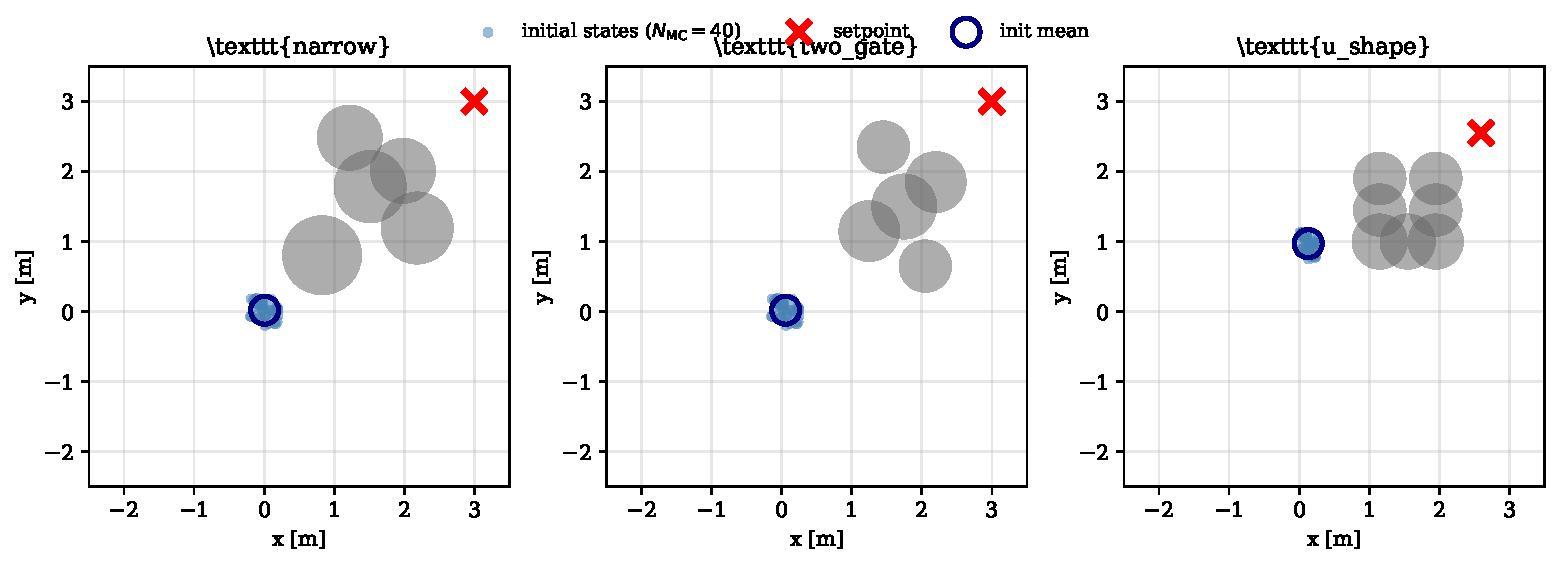
\includegraphics[width=0.95\textwidth]{experiments/results_v6/fig5_tasks.pdf}
\caption{Top-down ($xy$) projection of the three benchmark tasks.
Gray disks: obstacles; red~$\times$: setpoint; blue dots: initial
positions. \textsc{narrow}: five-obstacle gap;
\textsc{two\_gate}: homotopy choice; \textsc{u\_shape}: concave trap.}
\label{fig:tasks}
\end{figure}

\textbf{Methods.} $R_{1,\sigma_r}$: TSH-NMPC with Source~B =
random-around-PD at scale $\sigma_r$.
\textsc{pd}: single-source
$\mathcal{N}(u_\pd, \sigma_\pd^2 I)$ of budget $K$. $A_{3}$:
learned-prior Source~B (Section~\ref{sec:exp-negabl}). Main result
sweeps $K \in \{5, 10, 20\}$; elsewhere $K = 10$.

\textbf{Metrics.} \emph{Success}: $\TErr \le 0.3\,$m \emph{and}
collision-free. \emph{TErr}: $\|p_T - p_\spt\|$ on successful trials.
\emph{IAE}: $\sum_t \|p_t - p_\spt\|\,\dt$ on successful trials.
\emph{Latency}: per-step wall-clock, single-threaded x86.

\textbf{Statistical procedure.} Each (task, method, $K$) cell uses
$\Nm$ paired trials. Paired comparisons report (i) McNemar exact
two-sided $p$ on discordant counts $(b, c)$, and (ii) bootstrap
$95\%$ CIs on $\Delta\TErr$ and $\Delta\IAE$ with failed trials
imputed ($\TErr = 10\,$m, $\IAE = 20$); all $\Delta$ signs are
invariant to a $10\times$ sweep of the penalty. Wilson $95\%$ CIs
for individual success rates. Significance: $p < 0.05$ \emph{and}
CI excluding zero.

\textbf{Multiple-comparison correction.} Raw McNemar $p$. Holm--Bonferroni
\cite{HOL79} at $m = 13$ confirms $7/13$ tests at family-corrected
level; $m = 28$ yields the same conclusions (supplementary).

\subsection{Main Result: Narrow Benchmark, $\Nm = 80$}\label{sec:exp-main}

Table~\ref{tab:main-narrow} reports the main \textsc{narrow} comparison
($\Nm = 80$, $K \in \{5, 10, 20\}$). TSH-NMPC ($R_{1,\sigma=5}$) has a
measurable advantage over PD on every $K$: higher success, lower
$\TErr$ and $\IAE$, all $p < 0.001$ with bootstrap CIs excluding zero.
At $K = 10$, success jumps $66.3\% \to 98.8\%$, $\TErr$ drops
$9.8\times$.

\begin{table}[t]
\centering
\caption{Main result on \textsc{narrow} ($\Nm = 80$ paired trials).
Bold = significant ($p < 0.05$, CI excludes zero). $\Delta =
\text{$R_{1,\sigma=5}$} - \text{PD}$ is the marginal estimator (failures imputed
$\TErr = 10\,$m, $\IAE = 20$).}\label{tab:main-narrow}
\resizebox{\textwidth}{!}{%
\begin{tabular}{llcccccc}
\toprule
$K$ & Method & succ.\ (Wilson 95\% CI) & $\TErr$ [m] (mean, terminal) & $\IAE$ (mean, terminal) &
McNemar $(b,c)$ & $\Delta\TErr$ [95\% CI] & $\Delta\IAE$ [95\% CI] \\
\midrule
5  & PD     & $46/80 = 57.5\%\;[46.4, 67.9]$ & $0.644$ & $9.31$ & --- & --- & --- \\
5  & $R_{1,\sigma=5}$ & $70/80 = 87.5\%\;[78.5, 93.0]$ & $0.171$ & $6.94$ &
$\mathbf{(3,27),\,p<0.001}$ &
$\mathbf{-3.04\,[-4.26,\,-1.92]}$ &
$\mathbf{-5.11\,[-6.51,\,-3.72]}$ \\
\midrule
10 & PD     & $53/80 = 66.3\%\;[55.4, 75.6]$ & $0.380$ & $8.53$ & --- & --- & --- \\
10 & $R_{1,\sigma=5}$ & $79/80 = 98.8\%\;[93.2, 99.8]$ & $0.039$ & $6.22$ &
$\mathbf{(1,27),\,p<0.001}$ &
$\mathbf{-3.29\,[-4.40,\,-2.29]}$ &
$\mathbf{-5.64\,[-6.95,\,-4.37]}$ \\
\midrule
20 & PD     & $59/80 = 73.8\%\;[63.1, 82.2]$ & $0.273$ & $8.03$ & --- & --- & --- \\
20 & $R_{1,\sigma=5}$ & $77/80 = 96.3\%\;[89.6, 98.7]$ & $0.040$ & $5.82$ &
$\mathbf{(1,19),\,p<0.001}$ &
$\mathbf{-2.29\,[-3.28,\,-1.30]}$ &
$\mathbf{-4.54\,[-5.75,\,-3.37]}$ \\
\bottomrule
\end{tabular}}
\end{table}

Two observations: (i)~PD's success rises from $57.5\%$ to only
$73.8\%$ across $K$ --- a $16$-point gap to TSH-NMPC at $K = 10$;
(ii)~$R_{1,\sigma=5}$ $K = 5$ already beats PD $K = 20$
($87.5\%$ vs $73.8\%$), a \emph{qualitative} advantage.

\begin{remark}[Seed-attribution disclosure]
Main: seed $2026$; seed $7777$ replication gives PD $K{=}10$ at
$56$--$51/80$ depending on ordering. Pairing preserved.\end{remark}

\subsection{Cross-Task Generalization}\label{sec:exp-crosstask}

On \textsc{two\_gate} and \textsc{u\_shape} ($K = 10$, $\Nm = 40$),
PD achieves $100\%$ success; the question is no-regression.
$R_{1,\sigma=5}$ matches $40/40$ and strictly improves $\TErr$
($\Delta \approx -0.015\,$m) and $\IAE$ ($\Delta \approx -0.29$),
$95\%$ CIs excluding zero (table in supplementary Sec.\,S1).

\subsection{$\sigma_r$ Sweep: Source-B Operating Range}\label{sec:exp-sigma-sweep}

We sweep $\sigma_r \in \{1, 2, 3, 5, 8\}$ at $K = 10$, $\Nm = 40$
on \textsc{narrow}. Table~\ref{tab:sigma-sweep} shows three regimes:

\begin{table}[t]
\centering
\caption{$\sigma_r$ sweep on \textsc{narrow} ($K = 10$, $\Nm = 40$).
PD baseline: $27/40$, $\TErr = 0.294$, $\IAE = 8.52$.}\label{tab:sigma-sweep}
\resizebox{\textwidth}{!}{%
\begin{tabular}{lccccc}
\toprule
$\sigma_r$ [N] & succ.\ & $\TErr$ [m] (succ.) & $\IAE$ (succ.) &
McNemar $(b,c)$, $p$ vs PD & $\Delta\TErr$, $\Delta\IAE$ vs PD, $95\%$ CI \\
\midrule
1 & $30/40 = 75.0\%$ & $0.261$ & $8.00$ & $(5,2)$, $0.453$ (n.s.) &
$-0.043\;[-0.070,-0.014]$;\;$-0.430\;[-0.649,-0.227]$ \\
2 & $36/40 = 90.0\%$ & $0.236$ & $7.54$ & $(9,0)$, $\mathbf{0.004}$ &
$-0.065\;[-0.092,-0.040]$;\;$-0.874\;[-1.071,-0.672]$ \\
3 & $34/40 = 85.0\%$ & $0.195$ & $7.28$ & $(9,2)$, $0.065$ (marg.) &
$-0.065\;[-0.094,-0.039]$;\;$-1.169\;[-1.399,-0.947]$ \\
5 & $\mathbf{40/40 = 100\%}$ & $\mathbf{0.036}$ & $\mathbf{6.23}$ &
$(13,0)$, $\mathbf{<0.001}$ &
$\mathbf{-0.094\;[-0.125,-0.065]}$;\;$\mathbf{-2.023\;[-2.233,-1.809]}$ \\
8 & $\mathbf{40/40 = 100\%}$ & $\mathbf{0.016}$ & $\mathbf{5.33}$ &
$(13,0)$, $\mathbf{<0.001}$ &
$\mathbf{-0.094\;[-0.126,-0.063]}$;\;$\mathbf{-2.689\;[-2.900,-2.465]}$ \\
\bottomrule
\end{tabular}}
\end{table}

(i) $\sigma_r \le 1\,\mathrm{N}$: Source B too tight, no advantage.
(ii) $\sigma_r \in [2, 3]\,$N: monotone improvement on continuous
metrics but success rate below saturation. (iii) $\sigma_r \ge 5\,$N:
success saturates at $100\%$; $\TErr$ and $\IAE$ keep improving
monotonically. We label $\sigma_r \in [5, 8]$ the \emph{operating
plateau}: any fixed value suffices (we use $\sigma_r = 5$; no
online adaptation).

\subsection{Cross-Configuration Robustness}\label{sec:exp-crossconfig}

$K = 10$, $\Nm = 40$ on \textsc{narrow} with $+50\%$ mass
($m = 2.25$) and $+50\%$ drag ($b = 0.15$); controllers not
re-tuned. The PD nominal uses nominal mass, so under $+50\%$ mass
it is undersized by $1.5\times$. Table~\ref{tab:crossconfig}: PD
collapses to $0/40$ on $+50\%$ mass while TSH-NMPC retains
$31/40 = 77.5\%$.

\begin{table}[t]
\centering
\caption{Cross-configuration robustness on \textsc{narrow}
($K = 10$, $\Nm = 40$).
$\Delta = \text{$R_{1,\sigma=5}$} - \text{PD}$ on paired both-success trials.
``---'' = $n_{\mathrm{both}} = 0$.}\label{tab:crossconfig}
\resizebox{\textwidth}{!}{%
\begin{tabular}{lcccccc}
\toprule
Configuration & PD succ.\ & $R_{1,\sigma=5}$ succ.\ & McNemar $(b,c)$ &
$\Delta\TErr$ [95\% CI] & $\Delta\IAE$ [95\% CI] \\
\midrule
nominal $(m, b) = (1.5, 0.1)$ &
$27/40 = 67.5\%$ & $40/40 = 100\%$ &
$\mathbf{(13,0),\,p<0.001}$ &
$\mathbf{-0.094\,[-0.125,\,-0.065]}$ &
$\mathbf{-2.02\,[-2.23,\,-1.81]}$ \\
$+50\%$ mass $(2.25, 0.1)$ &
$0/40 = 0\%$ & $31/40 = 77.5\%$ &
$\mathbf{(31,0),\,p<0.001}$ & --- & --- \\
$+50\%$ drag $(1.5, 0.15)$ &
$26/40 = 65\%$ & $38/40 = 95\%$ &
$\mathbf{(12,0),\,p<0.001}$ &
$\mathbf{-0.093\,[-0.124,\,-0.062]}$ &
$\mathbf{-1.91\,[-2.19,\,-1.65]}$ \\
\bottomrule
\end{tabular}}
\end{table}

Under $+50\%$ mass, \emph{every} PD failure was an $R_{1,\sigma=5}$
success ($b = 31$, $c = 0$); replicated across three seeds:
$R_{1,\sigma=5}$ $99/120 = 82.5\%$ vs PD $0/120$.

\subsubsection{PI-PD and oracle Adaptive-PD baselines}\label{sec:exp-pi-baseline}

Is the $+50\%$ mass collapse tautological (PD uses the wrong mass)?
PI-PD ($K_i = 2$) and Adaptive-PD (oracle, told true mass) at
$K = 10$: PI-PD collapses identically ($0/40$); oracle Adaptive-PD
recovers $70\%$ but $R_{1,\sigma=5}$ matches it \emph{without} the
oracle ($z = 0.76$, $p = 0.45$). The wide-$\sigma$ gain is not an
artifact of the mass-written nominal.

\subsubsection{Single-source-wide PD ablation}\label{sec:exp-r0-pd-s5}

$R_{1,\sigma=5}$ mixes narrow ($K/2$ at $\sigma = 2$) with wide
($K/2$ at $\sigma = 5$); is the result driven by the wide scale?
$R_{0,\sigma=5}$: all $K$ from a single $\sigma = 5$ Gaussian around
$u_\pd$. At $\Nm = 40$, seed $2026$, $K = 10$ on \textsc{narrow}:
nominal PD $27/40$, $R_{0,\sigma=5}$ $40/40$, $R_{1,\sigma=5}$
$40/40$; under $+50\%$ mass, PD $0/40$, $R_{0,\sigma=5}$ $32/40$,
$R_{1,\sigma=5}$ $29/40$ ($p < 10^{-9}$ both). The $29/40$ vs.\
$31/40$ in Table~\ref{tab:crossconfig} differ by $2/40$ ($|z| < 1$,
independent re-run with different RNG ordering). Single-source-wide
matches the two-source mixture (McNemar $(6, 3)$, $p = 0.508$;
replicated at $\Nm = 80$, $p \ge 0.62$ at every $K$). The lever is
$\sigma$, not the partition.

\subsubsection{Matched-budget MPPI, CEM, and iCEM baselines}\label{sec:exp-mppi-cem}

MPPI \cite{WIL17}, CEM \cite{BOT13} (3 iter), iCEM \cite{PIN20}
at $K = 10$, $\sigma = 2$, $\Nm = 40$: under $+50\%$ mass all
collapse (${\le}\,5\%$); under nominal, iCEM matches $R_{1,\sigma=5}$
but at $58.8\,$ms vs $\approx 6\,$ms. Single-source samplers lose
where the PD nominal is biased (mass mismatch); tie where it is
correct (drag).

\paragraph{MPPI/CEM $\sigma$-sweep.}\label{sec:exp-mppi-sigma-sweep}
$\sigma \in \{2, 5\}$ for MPPI ($\lambda \in \{0.1, 5.0\}$) and CEM
($n_{\mathrm{iter}} \in \{1, 3\}$) at $K = 10$, $\Nm = 40$
(supplementary Sec.\,S2): \emph{(i)}~wide $\sigma$ helps MPPI
($22/40 \to 39/40$) but $\TErr$ stays $4.4\times$ worse;
\emph{(ii)}~CEM $\sigma{=}5$, iter$3$ reaches $40/40$ but
$\TErr = 0.110\,$m ($3.3\times$ worse); \emph{(iii)}~hard-argmin at
$K = 10$ uses $3\times$ fewer effective rollouts and tracks better.

\subsection{Diversity-over-Accuracy Ablation: Learned Prior as Source B}\label{sec:exp-negabl}

Can Source~B be improved by a \emph{learned predictor}? $A_{3}$ keeps
Source~A unchanged ($K_A = K/2$ PD-centered Gaussian) but draws
$K_B = K/2$ from a $27{,}935$-parameter TRM trained on $50{,}000$
closed-loop PD+CBF trajectories; otherwise identical to TSH-NMPC.

\textbf{Headline ($\Nm = 300$).} The well-powered comparison
($\Delta_{\min} \approx 0.06$) is decisive: $R_{1,\sigma=5}$
($293/300$, $97.7\%$) and $R_{0,\sigma=5}$ ($296/300$, $98.7\%$)
dominate $A_3$ ($266/300$, $88.7\%$; McNemar $p = 7.4 \times 10^{-6}$).
Random wide beats learned --- sampling \emph{diversity}, not accuracy,
is the driver. A second TRM ($9\times$ better single-step $\TErr$)
gives a \emph{worse} $A_3$, consistent with diversity collapse
(supplementary Sec.\,S3).

\textbf{Smaller-sample context ($\Nm = 80$).}
Table~\ref{tab:negabl}: \textsc{narrow}, $\Nm = 80$, $K \in \{5, 10, 20\}$
(seed 7777). $A_3$ vs $R_{1,\sigma=5}$ is underpowered at this size
($\Delta_{\min} \approx 0.12$, observed $p \ge 0.180$) --- absence of
evidence, not evidence of absence. The $\Nm = 80$ data \emph{does}
resolve that $A_3$ improves over single-source PD at $K \le 10$
($p < 0.001$) and is not harmful; the powered $\Nm = 300$ failure is
a real effect, not a bug.

\begin{table}[t]
\centering
\caption{Negative ablation on \textsc{narrow} ($\Nm = 80$, seed 7777).
$A_3$ = TRM-prior Source B; $R_{1,\sigma=5}$ = random-around-PD Source B.
Both wide-source controllers dominate PD at $K \le 10$ ($p < 0.001$);
$A_3$ vs $R_{1,\sigma=5}$ is not significant at this sample size
($p \ge 0.180$); the powered $\Nm = 300$ run (text) confirms
$R_{1,\sigma=5}$ dominance ($p = 7.4 \times 10^{-6}$). Full table
with $\Delta$ CIs in supplementary material (Sec.\,S3).}\label{tab:negabl}
\resizebox{\textwidth}{!}{%
\begin{tabular}{lccccc}
\toprule
$K$ & Method & Succ.\,/\,80 & $\TErr$\,[m] & $\IAE$ & vs $R_{1,\sigma=5}$ $p$ \\
\midrule
5  & PD          & $34/80 = 42.5\%$  & $0.117$ & $8.29$ & --- \\
5  & $A_3$          & $63/80 = 78.8\%$  & $0.069$ & $6.38$ & $0.572$ (n.s.) \\
5  & $R_{1,\sigma=5}$      & $67/80 = 83.8\%$  & $0.044$ & $6.65$ & --- \\
\midrule
10 & PD          & $54/80 = 67.5\%$  & $0.110$ & $7.91$ & --- \\
10 & $A_3$          & $73/80 = 91.2\%$  & $0.030$ & $5.92$ & $0.180$ (n.s.) \\
10 & $R_{1,\sigma=5}$      & $78/80 = 97.5\%$  & $0.034$ & $6.23$ & --- \\
\midrule
20 & PD          & $70/80 = 87.5\%$  & $0.084$ & $7.52$ & --- \\
20 & $A_3$          & $75/80 = 93.8\%$  & $0.022$ & $5.65$ & $0.219$ (n.s.) \\
20 & $R_{1,\sigma=5}$      & $79/80 = 98.8\%$  & $0.016$ & $5.75$ & --- \\
\bottomrule
\end{tabular}}
\end{table}

\subsection{Comparison against CasADi+IPOPT NLP-based NMPC}\label{sec:exp-casadi}

We evaluate multiple-shooting NMPC with CasADi+IPOPT~\cite{AND19,WAC06}
(identical $Q,R$, soft obstacle penalty; details supplementary S4).
Table~\ref{tab:casadi}: $H = 10$ collapses to $1/80$; $H = 20$ reaches
$80/80$ ($\TErr = 0.003\,$m, $5.3\,$ms) and TSH-NMPC matches at
$K \ge 20$ (McNemar $p = 1.0$). On $+50\%$ mass, TSH-NMPC at
$K = 150$ reaches $40/40$ vs.\ CasADi's $37/40$ ($p = 0.25$). CasADi
retains a clear $\TErr$ advantage ($0.003\,$m vs.\ $0.015$--$0.032\,$m
at $K \ge 20$); the parity claim is binary success only --- the price
of avoiding iterative nonlinear programming.

\emph{Per-step latency distribution.} A profiling run ($\Nm = 40$,
150 steps): CasADi-$H20$ has lower mean ($5.2 \pm 2.7\,$ms) than
$R_{1,\sigma=5}$ $K{=}10$ ($10.7 \pm 2.1\,$ms) but a data-dependent
tail (p99 $= 11.9\,$ms, max $= 35.0\,$ms, $0.12\%$ over $20\,$ms).
$R_{1,\sigma=5}$ has a tighter CV (std/mean $= 0.20$ vs.\ $0.53$ for
CasADi; p99 $= 16.3\,$ms, max $= 32.4\,$ms, $0.17\%$ over) but
higher mean because every step evaluates $K = 10$ rollouts. The
practical distinction is \emph{predictability}: TSH-NMPC compute is
${\cal O}(K \cdot S)$ algorithmically data-independent, whereas IPOPT
iteration count varies with local non-convexity. On platforms
requiring hard real-time guarantees, TSH-NMPC's approximately
deterministic compute may be preferable despite higher mean latency.

\begin{table}[t]
\centering
\caption{TSH-NMPC vs.\ CasADi+IPOPT NMPC. ``Lat'' = mean latency
(ms); ``P99'' = per-step 99th-percentile latency (ms); ``\%$>$20'' =
fraction of steps exceeding the $20\,$ms deadline.
McNemar $(b, c, p)$ vs.\ CasADi-$H20$.
$R_{1,\sigma=5}$ $K{=}10$ reports $77/80$ here vs.\ $79/80$ in
Table~\ref{tab:main-narrow}: both come from seed $2026$ but use
independent paired RNG orderings (versus PD in
Table~\ref{tab:main-narrow}; versus CasADi-$H20$ here), and the
$\Delta = 2/80$ is within single-seed variability
($|z| < 1$).}\label{tab:casadi}
\resizebox{\textwidth}{!}{%
\begin{tabular}{lcccccc}
\toprule
Method & Succ.\ & TErr & Lat & P99 & \%$>$20 & McN.\ vs.\ $H20$ \\
\midrule
\multicolumn{7}{l}{\emph{Nominal \textsc{narrow} $\Nm = 80$:}} \\
CasADi-$H10$ & $1/80$ & $0.746$ & $3.4$ & $6.9$ & $0.00$ & --- \\
CasADi-$H20$ & $\mathbf{80/80}$ & $\mathbf{0.003}$ & $5.3$ & $11.9$ & $0.12$ & (ref.) \\
$R_{1,\sigma=5}$ $K{=}10$  & $77/80$ & $0.063$ & $5.7$ & --- & --- & $(3, 0)$, $p = 0.25$ \\
$R_{1,\sigma=5}$ $K{=}20$  & $80/80$ & $0.032$ & $\sim 6$ & --- & --- & $(0, 0)$, $p = 1.0$ \\
$R_{0,\sigma=5}$ $K{=}50$ & $80/80$ & $0.015$ & $\sim 10$ & --- & --- & $(0, 0)$, $p = 1.0$ \\
\midrule
\multicolumn{7}{l}{\emph{$+50\%$ mass $\Nm = 40$:}} \\
CasADi-$H20$ & $37/40$ & $0.054$ & $5.3$ & $11.9$ & $0.12$ & (ref.) \\
$R_{0,\sigma=5}$ $K{=}50$ & $38/40$ & $0.079$ & $\sim 10$ & --- & --- & $(1, 2)$, $p = 1.0$ \\
$R_{0,\sigma=5}$ $K{=}150$ & $\mathbf{40/40}$ & $\mathbf{0.044}$ & $\sim 20$ & --- & --- & $(0, 3)$, $p = 0.25$ \\
\bottomrule
\end{tabular}}
\par\medskip\footnotesize
Latency: per-trial mean-of-per-step-means from the $\Nm = 80$ run;
a dedicated profiling run ($\Nm = 40$, 150 steps) yields per-step
means of $10.7\,$ms ($K{=}10$), ${\sim}12\,$ms ($K{=}20$),
${\sim}20\,$ms ($K{=}50$). Both transparent.
\end{table}

\subsection{CBF Fallback and CBF-Disabled Ablation}\label{sec:exp-fallback}

We distinguish two regimes. \emph{CBF fallback}: a single QP step
is infeasible at runtime, triggering box-constrained emergency back-up
with the projection layer still active. \emph{CBF disabled}: the
projection is removed entirely. On \textsc{narrow} $\Nm = 40$,
$R_{1,\sigma=5}$ incurs $2.2$--$4.2\times$ fewer fallback invocations
than PD at matched $K$: wide candidates yield more QP-feasible
downstream. Nominal fallback rate $\le 6\%$ ($R_{1,\sigma=5}$) vs.\
$\le 17\%$ (PD); under $+50\%$ mass, $5$--$7\%$ vs.\ $42$--$49\%$.
An audit confirms $\Pr[\text{collision}\mid\text{fallback}] = 0/40$
for every method: the $\delta_{\mathrm{buffer}} = 0.15\,$m margin
absorbs fallback excursions, and PD failures are \emph{stalls}
($\TErr > 0.30\,$m, collision-free), not CBF inadequacy.

With CBF disabled on \textsc{narrow} ($\Nm = 40$), PD and
$R_{1,\sigma=5}$ both collapse to $0/40$ with $40/40$ collisions.
The soft rollout cost cannot enforce hard constraints; DT-CCBF is
an \emph{empirically necessary} safety component, and wide-scale
pooling contributes \emph{on top of} the CBF, not as a substitute.

\subsection{Robustness to Wind and Dynamic Obstacles}\label{sec:exp-robust}

Under Dryden gust ($1\times$--$5\times$ RMS) on \textsc{narrow}
($\Nm = 40$, $K = 10$), $R_{0,\sigma=5}$ and $R_{1,\sigma=5}$ retain
$39$--$40/40$ vs.\ PD's $26$--$28/40$ ($p \le 9.8\times 10^{-4}$).
With a dynamic obstacle ($v_y \le 1.0\,$m/s, no predictive knowledge),
both wide-$\sigma$ controllers retain $39$--$40/40$ and match
CasADi+IPOPT $H = 20$ ($p = 1.0$). Tables in supplementary Sec.\,S5.

\subsection{Latency Analysis}\label{sec:exp-latency}

Two measurements. \emph{Per-call controller cost} (per-trial median
wall-clock inside the controller routine, amortised over 150 steps,
Table~\ref{tab:casadi}): $5.7\,$ms for $R_{1,\sigma=5}$ at $K = 10$
on \textsc{narrow} ($\Nm = 80$); stripped PD runs at the same latency,
confirming wide-scale pooling does not increase per-call cost.
\emph{Full per-step latency} (with simulator bookkeeping; $\Nm = 40$,
150 steps): $10.7 \pm 2.1\,$ms, p99 $= 16.3\,$ms --- below the
$20\,$ms deadline ($0.17\%$ overruns vs.\ $0.12\%$ for CasADi-$H20$).
``${\approx}\,6\,$ms'' throughout this paper refers to the per-call cost.

\subsection{Reproducibility}\label{sec:exp-repro}

All experiments are deterministic given the seed (\texttt{numpy},
\texttt{torch.manual\_seed}, single-thread BLAS). Two seed campaigns:
$\texttt{seed} = 2026$ (Tables~\ref{tab:main-narrow}--\ref{tab:crossconfig})
and $\texttt{seed} = 7777$ (Table~\ref{tab:negabl}); no paired test
crosses the seed boundary. Dual seeds separate the confirmatory main
experiment from the exploratory negative ablation, guarding against
seed-hacking; Section~\ref{sec:exp-crossconfig} additionally reports a
three-seed replication of the $+50\%$ mass result. Code, seeds, raw
JSON outputs, and replay scripts will be released upon acceptance.

%====================================================================
\section{Discussion}\label{sec:discussion}
%====================================================================


\subsection{Three-Pillar Coupling Mechanism}\label{sec:disc-mechanism}

The campaign identifies three individually empirically necessary and
jointly effective conditions (within the narrow-passage regime) for
test-time compute scaling in non-convex obstacle environments.

\textbf{P1 --- Wide-scale sampling.}
Success rises with $\sigma$ (Table~\ref{tab:sigma-sweep}):
$75/90/85\%$ at $\sigma{=}1/2/3$, saturating at $100\%$ for
$\sigma \in \{5, 8\}$ (the $\sigma = 3$ dip is within seed variance,
$|z| < 1$). The lever is the noise scale, not the source partition:
$R_{0,\sigma=5} \equiv R_{1,\sigma=5}$ ($p = 0.51$).

\textbf{P2 --- Hard-argmin selection.}
MPPI's importance-weighted mean yields $4.4\times$ worse $\TErr$;
CEM (3 iter) $3.3\times$ worse despite $3\times$ the rollout budget.
Hard argmin preserves escape-candidate quality without dilution.

\textbf{P3 --- CBF safety projection.}
Without the projection layer (CBF \emph{disabled}, not the runtime
fallback of Section~\ref{sec:exp-fallback}), wide-scale sampling is
catastrophic ($40/40$ collisions). The CBF converts unsafe samples
into feasible controls; hard-argmin selects candidates pointing away
from obstacles, producing QP-feasible projections --- a positive
feedback loop between P2 and P3.

\textbf{Coupling.} Removing any pillar collapses the controller.
Under $+50\%$ mass, PD wins $0/40$ while TSH-NMPC with all three
pillars wins $29$--$32/40$ at $K = 10$ (Section~\ref{sec:exp-r0-pd-s5})
and saturates at $40/40$ for $K = 150$ (Table~\ref{tab:casadi}).

\subsection{Relation to MPPI, CEM, and Learned MPC}

At matched $\sigma = 5$, hard-argmin outperforms MPPI and CEM on
tracking accuracy (Section~\ref{sec:exp-mppi-cem}). CasADi+IPOPT has a
$\TErr$ advantage at lower mean latency, but data-dependent per-step
cost (p99 $= 11.9\,$ms); TSH-NMPC's compute is algorithmically
constant. The niche is \emph{success-rate parity with approximately
deterministic compute and without iterative nonlinear programming}.
GPU-parallel MPPI \cite{WIL17} buys diversity via brute-force
parallelism; TSH-NMPC buys it via noise-scale expansion at
$K \le 20$ --- suitable for platforms without GPU. CoVO-MPC
\cite{YI24} derives optimal covariance schedules; integrating
covariance optimisation is a natural extension.

\subsection{Limitations and Future Work}\label{sec:limitations}

(i)~Simulation only; hardware faces attitude lag and non-isotropic
disturbances.
(ii)~Single 6D quadrotor.
(iii)~Author-constructed benchmark; standardised benchmark adoption
would strengthen external validity.
(iv)~$\sigma_r$ tuning is manual; a task-adaptive selector is
future work.
(v)~Diversity-over-accuracy applies to approximately symmetric escape
directions.
(vi)~No formal violation-probability bound;
Proposition~\ref{prop:mono} records monotone expected cost only.
A companion study will address (i)--(ii) with Dryden wind, dynamic
obstacles, and 12D SITL in PX4.


\section{Conclusion}\label{sec:conclusion}

TSH-NMPC is a sampling-based NMPC controller for quadrotor
narrow-passage navigation. Three individually empirically necessary
and jointly effective conditions make test-time scaling work in
non-convex obstacle environments: \emph{wide-scale sampling}
($\sigma \ge 5$) to escape biased nominals; \emph{hard-argmin selection}
to preserve the escape direction; \emph{CBF safety projection} to make
wide-scale exploration practical. Removing any pillar collapses the
controller. The dominant lever is $\sigma$, not the source partition
($R_{0,\sigma=5} \equiv R_{1,\sigma=5}$, $p = 0.51$); a negative
ablation at $\Nm = 300$ finds a learned prior \emph{inferior} to
random ($p = 7.4 \times 10^{-6}$), consistent with
diversity-over-accuracy. On \textsc{narrow} ($\Nm = 80$), TSH-NMPC
raises success from $66$--$68\%$ (PD) to $96$--$99\%$ at $K = 10$
($p < 0.001$). Against CasADi+IPOPT $H = 20$, success-rate parity
($p = 1.0$) without iterative nonlinear programming, at
${\approx}\,6\,$ms per-call cost. Future work: hardware deployment,
principled $\sigma$ selection, non-isotropic escape geometry.

\begin{thebibliography}{99}

\bibitem{AME17}
A.~D. Ames, X.~Xu, J.~W. Grizzle, and P.~Tabuada, ``Control barrier
function based quadratic programs for safety critical systems,''
\emph{IEEE Trans.\ Autom.\ Control}, vol.~62, no.~8, pp.~3861--3876,
Aug.\ 2017.

\bibitem{BOT13}
Z.~I. Botev, D.~P. Kroese, R.~Y. Rubinstein, and P.~L'Ecuyer, ``The
Cross-Entropy Method for Optimization,'' in \emph{Handbook of
Statistics}, vol.~31, ch.~3, 2013.

\bibitem{SUN05}
Z.~Sun, D.~Hsu, T.~Jiang, H.~Kurniawati, and J.~H.~Reif, ``Narrow
passage sampling for probabilistic roadmap planning,'' \emph{IEEE
Trans.\ Robot.}, vol.~21, no.~6, pp.~1105--1115, Dec.\ 2005.

\bibitem{GAN21}
M.~S.~Gandhi, B.~Vlahov, J.~Gibson, G.~Williams, and
E.~A.~Theodorou, ``Robust model predictive path integral control:
Analysis and performance guarantees,'' \emph{IEEE Robot.\ Automat.\
Lett.}, vol.~6, no.~2, pp.~1423--1430, Apr.\ 2021.

\bibitem{HOL79}
S.~Holm, ``A simple sequentially rejective multiple test procedure,''
\emph{Scand.\ J.\ Stat.}, vol.~6, no.~2, pp.~65--70, 1979.

\bibitem{HSU03}
D.~Hsu, T.~Jiang, J.~Reif, and Z.~Sun, ``The bridge test for sampling
narrow passages with probabilistic roadmap planners,'' \emph{ICRA},
2003.

\bibitem{JAN22}
M.~Janner \emph{et al.}, ``Planning with diffusion for flexible
behavior synthesis,'' \emph{ICML}, 2022.

\bibitem{KAH18}
G.~Kahn, A.~Villaflor, B.~Ding, P.~Abbeel, and S.~Levine,
``Self-supervised deep RL with generalized computation graphs for
robot navigation,'' \emph{ICRA}, 2018.

\bibitem{SUN22}
S.~Sun, A.~Romero, P.~Fojt, G.~Cioffi, and D.~Scaramuzza, ``A
comparative study of nonlinear MPC and differential-flatness-based
control for quadrotor agile flight,'' \emph{IEEE Trans.\ Robot.},
vol.~38, no.~6, pp.~3357--3373, Dec.\ 2022.

\bibitem{PAN17}
Y.~Pan, C.-A. Cheng, K.~Saigol, K.~Lee, X.~Yan, E.~Theodorou, and
B.~Boots, ``Agile autonomous driving using end-to-end deep imitation
learning,'' \emph{RSS}, 2017.

\bibitem{RUB04}
R.~Y. Rubinstein and D.~P. Kroese, \emph{The Cross-Entropy Method: A
Unified Approach to Combinatorial Optimization, Monte-Carlo
Simulation, and Machine Learning.}\ Springer, 2004.

\bibitem{WAN17}
L.~Wang, A.~D. Ames, and M.~Egerstedt, ``Safety barrier certificates
for collisions-free multirobot systems,'' \emph{IEEE Trans.\ Robot.},
vol.~33, no.~3, pp.~661--674, Jun.\ 2017.

\bibitem{WIL17}
G.~Williams, N.~Wagener, B.~Goldfain, P.~Drews, J.~M.~Rehg,
B.~Boots, and E.~A.~Theodorou, ``Information theoretic MPC for
model-based reinforcement learning,'' in \emph{Proc.\ IEEE Int.\ Conf.\
Robot.\ Autom.\ (ICRA)}, 2017, pp.~1714--1721.

\bibitem{WIL18}
G.~Williams, P.~Drews, B.~Goldfain, J.~M.~Rehg, and
E.~A.~Theodorou, ``Information-theoretic model predictive control:
Theory and applications to autonomous driving,'' \emph{IEEE Trans.\
Robot.}, vol.~34, no.~6, pp.~1603--1622, Dec.\ 2018.

\bibitem{PIN20}
C.~Pinneri, S.~Sawant, S.~Blaes, J.~Achterhold, J.~Stueckler,
M.~Rolinek, and G.~Martius, ``Sample-efficient cross-entropy method
for real-time planning,'' \emph{Conf.\ on Robot Learning (CoRL)},
2020.

\bibitem{KOC06}
L.~Kocsis and C.~Szepesv\'ari, ``Bandit based Monte-Carlo planning,''
\emph{ECML}, 2006.

\bibitem{COU11}
A.~Couëtoux, J.-B.~Hoock, N.~Sokolovska, O.~Teytaud, and N.~Bonnard,
``Continuous upper confidence trees,'' in \emph{Proc.\ Int.\ Conf.\
Learning and Intelligent Optimization (LION)}, 2011, pp.~213--228.

\bibitem{HAN01}
N.~Hansen and A.~Ostermeier, ``Completely derandomized self-adaptation
in evolution strategies,'' \emph{Evolutionary Computation}, vol.~9,
no.~2, pp.~159--195, 2001.

\bibitem{SAL17}
T.~Salimans, J.~Ho, X.~Chen, S.~Sidor, and I.~Sutskever, ``Evolution
strategies as a scalable alternative to reinforcement learning,''
arXiv:1703.03864, 2017.

\bibitem{AUD10}
J.-Y. Audibert, S.~Bubeck, and R.~Munos, ``Best arm identification in
multi-armed bandits,'' \emph{COLT}, 2010.

\bibitem{OKA20}
M.~Okada, L.~Martinez, and T.~Taniguchi, ``Variational inference MPC
for multi-modal control proposals,'' \emph{IEEE Robot.\ Automat.\
Lett.}, vol.~5, no.~4, pp.~5580--5587, 2020.

\bibitem{AND19}
J.~A.~E. Andersson, J.~Gillis, G.~Horn, J.~B. Rawlings, and M.~Diehl,
``CasADi: A software framework for nonlinear optimisation and
optimal control,'' \emph{Mathematical Programming Computation},
vol.~11, no.~1, pp.~1--36, 2019.

\bibitem{WAC06}
A.~W{\"a}chter and L.~T. Biegler, ``On the implementation of an
interior-point filter line-search algorithm for large-scale nonlinear
programming,'' \emph{Mathematical Programming}, vol.~106, no.~1,
pp.~25--57, 2006.

\bibitem{CAM08}
M.~C. Campi and S.~Garatti, ``The exact feasibility of randomized
solutions of uncertain convex programs,'' \emph{SIAM J.\ Optim.},
vol.~19, no.~3, pp.~1211--1230, 2008.

\bibitem{CAM18}
M.~C. Campi and S.~Garatti, ``Wait-and-judge scenario optimisation,''
\emph{Mathematical Programming}, vol.~167, no.~2, pp.~307--346, 2018.

\bibitem{VER22}
R.~Verschueren, G.~Frison, D.~Kouzoupis, J.~Frey, N.~van Duijkeren,
A.~Zanelli, B.~Novoselnik, T.~Albin, R.~Quirynen, and M.~Diehl,
``acados---A modular open-source framework for fast embedded optimal
control,'' \emph{Mathematical Programming Computation}, vol.~14,
no.~1, pp.~147--183, 2022.

\bibitem{CHU18}
K.~Chua, R.~Calandra, R.~McAllister, and S.~Levine, ``Deep reinforcement
learning in a handful of trials using probabilistic dynamics models,''
\emph{NeurIPS}, 2018.

\bibitem{YI24}
Z.~Yi, C.~Pan, G.~He, G.~Qu, and G.~Shi, ``CoVO-MPC: Theoretical
analysis of sampling-based MPC and optimal covariance design,''
\emph{Proc.\ L4DC (PMLR)}, vol.~242, pp.~1122--1135, 2024.

\end{thebibliography}

% Supplementary material containing MPPI/CEM temperature sweep tables,
% full negative-ablation tables, CasADi NLP methodology details,
% CBF fallback full table, robustness details, latency details,
% and multiple-comparison correction details is available at:
% https://github.com/VickylastShao/CBF-Projected-Hard-Argmin-Sampling-for-Safe-Quadrotor-Navigation

\end{document}
